\chapter{Previous Searches}
As mentioned above, there are many theoretical motivations to study final states at the LHC involving h+\ptmiss. These final states provide some of the best ways to further constrain the parameter space offered by a wide variety of simplified DM models. Studying this final state can help lead to conclusions about the viability of indirect DM detection of these models. One subset of h+\ptmiss searches are those involving decays of the observed Higgs to a b quark-antiquark pair. This is a useful decay to look at because it is the most common Higgs decay~\cite{Zyla:2020zbs}. Another common Higgs decay to observe is h $\to\gamma\gamma$, since the di-photon decay tends to stand out background processes, even if it occurs at a much less frequent rate.

There have been several experimental searches for this state at the LHC. In one recent analysis, the CMS Collaboration used $\fbinv{35.9}$ of data collected in 2016 to search for dark matter in association with h $\to$ b$\bar{\mathrm{b}}$ decays~\cite{cms:hbb2019}. This search was motivated by the possibility of a coupling between the Higgs and theorized particles that would also couple to the DM sector, allowing further probing of DM-SM coupling. The search was analyzed through two frameworks. In the first, the observed Higgs is assumed to be the CP-even scalar h of the 2HDM+a model discussed in \cref{section:2hdma}. In the second framework, the observed Higgs interacts with a Z$'$ gauge boson that can decay to a dark matter candidate, as described in \cref{section:Z'}.

The analysis used the particle-flow (PF) algorithm~\cite{cms:pf2017} for object reconstruction. In order to find suitable Higgs candidates, the Cambridge-Aachen algorithm~\cite{cms:2009lxa} with distance parameter 1.5 was used to reconstruct jets likely produced by multiple quarks (CA15 jets), such as the two b quarks decaying from the Higgs. The analysis also formed jet objects using the anti-$k_{T}$ algorithm~\cite{ak2008} with a distance parameter of 0.4. The pileup per particle identification (PUPPI) algorithm~\cite{puppi2014} was used to avoid issues arising from pileup. The mass of the jet is calculated after using the soft-drop (SD) jet grooming algorithm~\cite{sd2014}. The final main variable used with the CA15 jets was a modified tagging variable N$_2^\text{DDT}$. The analysis identified several lepton objects through kinematic variables and identification requirements for use in eliminating background events. Here, the \ptvecmiss is calculated as the negative vector sum of the \pt of all reconstructed PF objects.

In order to focus in on the aforementioned final state, the analysis looked at events with high \ptmiss, no leptons or photons, and a CA15 jet. The analysis also defined several control regions in order to estimate the \ptmiss distribution of the main background processes, which are Z bosons produced in association with initial state jets, W bosons produced in association with initial state jets, and t$\bar{\mathrm{t}}$.
In all regions, it was required that the CA15 jet have $\pt > 200$ GeV, $|\eta| <2.4$, $100<m_{\text{SD}}<\GeV{200}$, and N$_2^\text{DDT} < 0$. There was also a requirement that the \ptmiss be greater than \GeV{200}. Finally, there were requirements that the azimuthal angle $\varphi$ between the AK4 jets and the \ptmiss be greater than 0.4 and that there were fewer than 2 AK4 jets with $R$ between them and the CA15 jet greater than 1.5.

The signal and background contributions were extracted with a simultaneous binned likelihood fit.
A variety of systematic uncertainties were assigned as nuisances, including b quark tagging/mistagging efficiencies, transfer factor statistical uncertainties, and the CA15 jet energy. No significant excess over the SM expectation was observed.

Using the 2HDM+a model, the analysis scanned and found excluded regions for $m_\mathrm{A}$, $\sin\theta$, and $\tan\beta$. With $\sin\theta=0.35$, $\tan\beta = 1$, $m_\mathrm{a}=\GeV{150}$, $m_\chi = \GeV{10}$, and $m_\mathrm{A}=m_\mathrm{H}=m_{\mathrm{H}^{\pm}}$, $m_\mathrm{A}$ between $500$ and $\GeV{900}$ are excluded. With $\tan\beta = 1$, $m_\mathrm{a}=\GeV{200}$, $m_\chi = \GeV{10}$, and $m_\mathrm{A}=m_\mathrm{H}=m_{\mathrm{H}^{\pm}} = \GeV{600}$, $\sin\theta$ between 0.35 and 0.75 are excluded. Finally, with $\sin\theta=0.35$, $m_\mathrm{a}=100$ ($150$) $\GeV{}$, $m_\chi = \GeV{10}$, and $m_\mathrm{A}=m_\mathrm{H}=m_{\mathrm{H}^{\pm}} = \GeV{600}$, $\tan\beta$ between 0.5 and 2.0 (1.6) are excluded. A summary of these results can be seen in \cref{fig:hbbmet20191}.

\begin{figure}[ht]
\centering
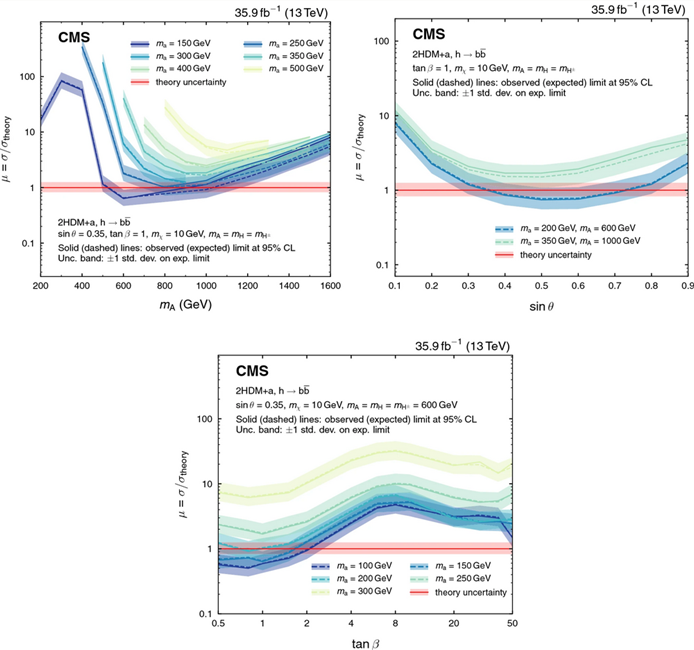
\includegraphics[width=0.8\textwidth]{Chapters/Experiment/2019hbbmet_results.png}
\caption{Upper limits on the 2HDM+a model of DM production in association with h $\to$ b$\bar{\mathrm{b}}$+\ptmiss obtained in~\cite{cms:hbb2019}. The theory uncertainty has been taken to be 20\%.}
\label{fig:hbbmet20191}
\end{figure}

Using the \Zp model, the analysis scanned and found excluded regions for $m_\Zp$ and $m_\chi$. For $m_\chi = \GeV{1}$, $m_\Zp$ is excluded up to $\GeV{1600}$. On the other hand, for $m_\Zp = \GeV{960}$, $m_\chi$ is excluded up to $\GeV{430}$. A summary of these results can be seen in \cref{fig:hbbmet20192}.

\begin{figure}[ht]
\centering
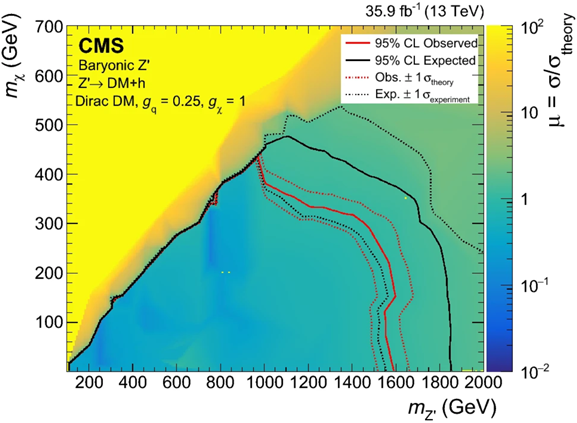
\includegraphics[width=0.6\textwidth]{Chapters/Experiment/2019hbbmet_results2.png}
\caption{Upper limits on the baryonic Z$'$ model of DM production in association with h $\to$ b$\bar{\mathrm{b}}$+\ptmiss obtained in~\cite{cms:hbb2019}.}
\label{fig:hbbmet20192}
\end{figure}

The ATLAS collaboration has published a couple of analyses examining the h $\to$ b$\bar{\mathrm{b}}$+\ptmiss final states in recent years, first using data gathered early in Run 2 of the LHC and then with the full dataset~\cite{atlas:hbb2017,atlas:hbb2021}. The latter search was interpreted through the 2HDM+a model as well as a model with an additional Higgs doublet and a \Zp boson.

For the 2HDM+a scenario, the $m_\mathrm{A}$-$m_\mathrm{a}$ parameter space was scanned for two values of $\tan\beta$. As mentioned in \cref{section:2hdma}, for smaller values of $\tan\beta$, the A pseudoscalar is most likely to couple to ah and t$\bar{\mathrm{t}}$. However, for larger values of $\tan\beta$, A is more likely to couple to b$\bar{\mathrm{b}}$. Thus, by scanning the parameter space with $\tan\beta=1$, events are more likely to be produced by gluon-gluon fusion, while scanning the space with $\tan\beta=10$ leads to more events produced by b$\bar{\mathrm{b}}$. For the gg ($\tan\beta=1$) initial state, with $g_\chi = 1$, $\sin\theta=0.35$, $m_\chi=\GeV{10}$, and $m_\mathrm{A}=m_\mathrm{H}=m_{\mathrm{H}^\pm}$ for $m_\mathrm{A}=\GeV{900}$, masses of a were excluded up to $\GeV{240}$, representing an improvement on previous results. For the b$\bar{\mathrm{b}}$ ($\tan\beta=10$) initial state, with $g_\chi = 1$, $\sin\theta=0.35$, $m_\chi=\GeV{10}$, and $m_\mathrm{A}=m_\mathrm{H}=m_{\mathrm{H}^\pm}$ for $m_\mathrm{A}=\GeV{1250}$, masses of a were excluded up to $\GeV{250}$, which are the first bounds established for these parameters. These results are pictured in \cref{fig:hbbmet20211}.

\begin{figure}[ht]
\centering
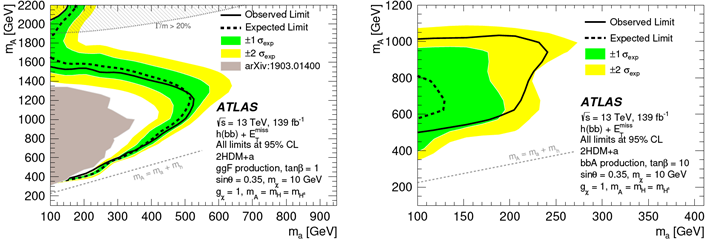
\includegraphics[width=\textwidth]{Chapters/Experiment/2021hbbmet_results.png}
\caption{Upper limits on the 2HDM+a model of DM production in association with h $\to$ b$\bar{\mathrm{b}}$+\ptmiss obtained in~\cite{atlas:hbb2021}. The solid (dashed) black lines give the observed 95\% CL (expected) limit, with the green and yellow bands giving the $1\sigma$ and $2\sigma$ uncertainties on the expected limit.}
\label{fig:hbbmet20211}
\end{figure}

For the \Zp-2HDM scenario, the $m_{\mathrm{A}^0}$-$m_\chi$ parameter space was scanned, with $g_z$ set to 0.8, $g_\chi=1$, $\tan\beta=1$, $m_\chi = \GeV{100}$, and $m_{\mathrm{A}^0}=m_\mathrm{H}=m_{\mathrm{H}^\pm}$. For $m_{\mathrm{A}^0} = \GeV{300}$, $m_\Zp$ values are excluded up to $\GeV{3000}$. These results are pictured in \cref{fig:hbbmet20212}.

\begin{figure}[ht]
\centering
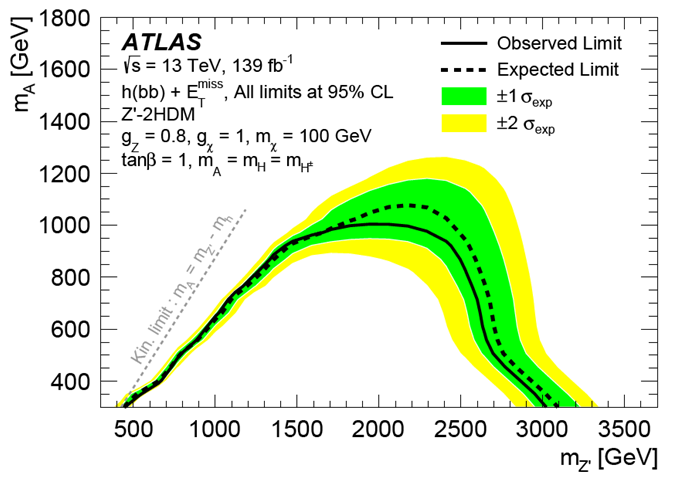
\includegraphics[width=0.6\textwidth]{Chapters/Experiment/2021hbbmet_results2.png}
\caption{Upper limits on the Z$'$-2HDM model of DM production in association with h $\to$ b$\bar{\mathrm{b}}$+\ptmiss obtained in~\cite{atlas:hbb2021}. The solid (dashed) black lines give the observed 95\% CL (expected) limit, with the green and yellow bands giving the $1\sigma$ and $2\sigma$ uncertainties on the expected limit.}
\label{fig:hbbmet20212}
\end{figure}